% !TeX program = xelatex
% 目录和交叉引用至少需要连续编译两次；推荐在提交包根目录运行“编译报告.ps1”。
\documentclass[UTF8,a4paper,12pt]{ctexart}

\usepackage[margin=2.5cm]{geometry}
\usepackage{amsmath,amssymb,bm}
\usepackage{booktabs,array}
\usepackage{graphicx,float,caption}
\usepackage{xcolor,hyperref}
\usepackage{siunitx}
\usepackage{fancyhdr}

\DeclareSIUnit\pixel{px}
\sisetup{detect-all}
\captionsetup{font=small,labelfont=bf}
\hypersetup{colorlinks=true,linkcolor=blue!55!black,urlcolor=blue!55!black,
  pdftitle={单图消失点与消失线标定实验报告}}

\newcommand{\StudentName}{贾宇航}
\newcommand{\StudentID}{26125201}
\newcommand{\CourseName}{机器视觉}

% 页眉：左侧为课程名称，中间为当前章节，右侧为页码。
\setlength{\headheight}{15pt}
\pagestyle{fancy}
\fancyhf{}
\fancyhead[L]{\CourseName}
\fancyhead[C]{\nouppercase{\leftmark}}
\fancyhead[R]{\thepage}
\renewcommand{\headrulewidth}{0.4pt}
\renewcommand{\footrulewidth}{0pt}
\renewcommand{\sectionmark}[1]{\markboth{#1}{}}
\fancypagestyle{plain}{
  \fancyhf{}
  \fancyhead[L]{\CourseName}
  \fancyhead[C]{\nouppercase{\leftmark}}
  \fancyhead[R]{\thepage}
  \renewcommand{\headrulewidth}{0.4pt}
  \renewcommand{\footrulewidth}{0pt}
}

\title{单图消失点与消失线标定实验报告}
\author{课程：\CourseName\qquad \StudentName\quad 学号：\StudentID}
\date{\today}

\begin{document}
\maketitle
\thispagestyle{empty}

\begin{abstract}
本实验从单幅棋盘格图像中提取两组互相正交的平行线，通过总体最小二乘和奇异值分解估计两个消失点及棋盘平面的消失线。在主点位于图像中心、像素轴倾斜为零且 $f_x=f_y$ 的先验下，进一步估计焦距和相机相对棋盘坐标系的旋转。最终选定图像为 \texttt{19/88.jpg}，得到焦距 \SI{320.962}{\pixel}，平均直线共点残差为 \SI{0.813}{\pixel}。实验同时说明：消失点只包含方向信息，不能单独恢复相机平移和绝对尺度；原图的径向畸变及远消失点会造成显著系统误差。

\textbf{关键词：}消失点；消失线；单图标定；正交约束；相机旋转
\end{abstract}

\clearpage
\tableofcontents
\clearpage

\section{实验目的}

\begin{enumerate}
  \item 从单幅图像中的两组平行线估计消失点和棋盘平面的消失线；
  \item 在明确内参先验的条件下估计相机焦距和相对棋盘的旋转；
  \item 分析双消失点法的可观测性、误差来源和适用范围；
  \item 给出可复现的消失点标定代码。
\end{enumerate}

\section{理论基础}

\subsection{消失点与正交约束}

设世界方向为 $\bm d_i$，其图像消失点满足
\begin{equation}
  \bm v_i\sim KR\bm d_i.
\end{equation}
若两个世界方向正交，则
\begin{equation}
  \bm v_x^T\omega\bm v_y=0,
  \qquad \omega=K^{-T}K^{-1}.
\end{equation}
单幅图像中的一对正交消失点只提供一个关于内参的独立约束，不能无条件求出一般的内参矩阵。为使问题可解，本实验采用以下假设：
\begin{itemize}
  \item 主点等于图像中心 $\bm c=(360,288)^T$；
  \item 像素轴倾斜为零；
  \item 方形像素，即 $f_x=f_y=f$；
  \item 棋盘的两个方向在三维空间中严格正交。
\end{itemize}
此时
\begin{equation}
  K=\begin{bmatrix}
  f&0&c_x\\
  0&f&c_y\\
  0&0&1
  \end{bmatrix},
\end{equation}
并有
\begin{equation}
  f=\sqrt{-\left[(u_x-c_x)(u_y-c_x)+(v_x-c_y)(v_y-c_y)\right]}.
  \label{eq:focal}
\end{equation}
根号内必须为正，否则说明消失点、正交关系或内参假设不一致。

\subsection{消失线与旋转}

棋盘平面的消失线为
\begin{equation}
  \bm l_{\infty}=\bm v_x\times\bm v_y.
\end{equation}
求得 $K$ 后，两个棋盘轴在相机坐标系中的单位方向为
\begin{equation}
  \bm r_i=\frac{K^{-1}\bm v_i}{\lVert K^{-1}\bm v_i\rVert}.
\end{equation}
令 $\bm r_3=\bm r_1\times\bm r_2$，并通过 SVD 投影到最近的合法旋转矩阵，可构造
\begin{equation}
  R=[\bm r_1\ \bm r_2\ \bm r_3].
\end{equation}
齐次消失方向存在正负号歧义，因此世界轴符号需结合棋盘坐标定义解释。

消失点表示无穷远方向，其投影关系中不含平移 $\bm t$，所以仅凭消失点不能恢复相机平移和绝对尺度。若要求平移，必须增加已知长度、已知三维点或相机高度等度量信息。

\section{实验方案与实现}

\subsection{直线拟合与消失点估计}

程序执行以下步骤：
\begin{enumerate}
  \item 在 $720\times576$ 像素图像中检测 $6\times4$ 个棋盘内角点，并进行亚像素优化；
  \item 将角点重排为 4 行、6 列，分别对每行和每列角点拟合直线 $au+bv+c=0$；
  \item 拟合前对坐标做中心化和尺度归一化，使用总体最小二乘求直线；
  \item 将同一方向的多条直线叠成矩阵，使用 SVD 求最小奇异值对应的齐次交点；
  \item 由式~\eqref{eq:focal} 计算焦距，并检查结果的数值有效性；
  \item 由两个消失点求消失线、内参矩阵和旋转矩阵。
\end{enumerate}

\subsection{单图候选选择}

自动检测会遍历编号目录中的候选图像。候选必须满足
\begin{equation}
  0.15W\leq f\leq2.5W,
\end{equation}
其中 $W=720$，即焦距接受范围为 $[108,1800]$ 像素。对每个候选计算
\begin{equation}
  S=\bar e_{\mathrm{con}}+0.0004\left(
  \lVert\bm v_x-\bm c\rVert_2+\lVert\bm v_y-\bm c\rVert_2\right),
\end{equation}
其中 $\bar e_{\mathrm{con}}$ 是各拟合直线到相应消失点的平均距离。选择 $S$ 最小的图像，以兼顾直线交会一致性并避免数值上过远的消失点。该评分含经验权重，因此它会影响最终候选选择，并不等价于独立精度验证。

\section{实验结果}

\subsection{单张消失线标定图片}

最终选定图像为 \texttt{19/88.jpg}。原图位于本文件夹的
\texttt{单张消失线原始图片} 子目录中。图~\ref{fig:vp} 中，红、绿直线分别表示棋盘的两个正交方向，白点为参与拟合的亚像素角点。

\begin{figure}[H]
  \centering
  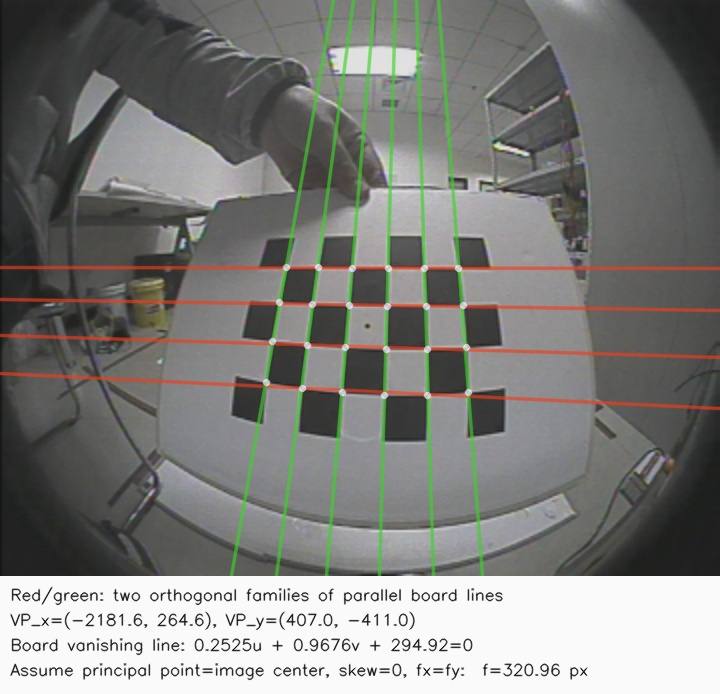
\includegraphics[width=0.82\textwidth]{单张消失线标定图.jpg}
  \caption{单幅图像中的两组直线及消失线标定结果}
  \label{fig:vp}
\end{figure}

\subsection{消失点、消失线和内参}

两组直线的消失点为
\begin{align}
  \bm v_x&=(-2181.5654,\ 264.6063,\ 1)^T,\\
  \bm v_y&=(406.9668,\ -411.0221,\ 1)^T.
\end{align}
平均直线共点残差为 \SI{0.813}{\pixel}。由正交约束得到
\begin{equation}
  f=\SI{320.9616}{\pixel},
  \qquad
  K=\begin{bmatrix}
  320.9616&0&360\\
  0&320.9616&288\\
  0&0&1
  \end{bmatrix}.
\end{equation}

归一化棋盘平面消失线为
\begin{equation}
  \bm l_{\infty}=(0.25255,\ 0.96758,\ 294.92015)^T,
\end{equation}
即
\begin{equation}
  0.25255u+0.96758v+294.92015=0.
\end{equation}
该直线位于当前画面之外，这与两个有限消失点的位置和棋盘平面朝向一致。

\subsection{旋转矩阵}

以棋盘两轴作为世界坐标系的前两轴，得到世界到相机坐标系的旋转矩阵
\begin{equation}
  R=\begin{bmatrix}
  -0.99208&0.06095&0.10984\\
  -0.00913&-0.90709&0.42083\\
  0.12528&0.41650&0.90046
  \end{bmatrix}.
\end{equation}
恢复出的两个方向点积绝对值为 $6.94\times10^{-18}$。由于焦距正是由同一对消失点的正交公式计算，该数值只能说明公式实现和浮点计算内部一致，不能视为独立精度证据。

\section{结果分析}

\begin{itemize}
  \item \SI{0.813}{\pixel} 的共点残差说明所选直线具有较好的交会一致性，但它使用了同一组拟合数据，并非独立验证误差。
  \item 一个消失点位于 $u=-2181.6$ 附近，距离图像很远。线方向的微小扰动会在交点位置上被大幅放大，使焦距对角点噪声较敏感。
  \item 原图具有明显径向畸变，真实空间直线在图像中并不严格为直线。直接拟合原始角点会给消失点和焦距带来系统偏差。
  \item 主点固定在图像中心且强制 $f_x=f_y$ 是使双消失点问题可解的关键先验；若实际相机不满足这些条件，结果会出现偏差。
  \item 两个正交方向足以构造完整旋转，但方向符号需要结合世界轴定义确定。平移和绝对尺度仍不可观测。
  \item 提高精度的方法包括：先进行独立去畸变、使用 RANSAC 剔除异常线段、增加第三个两两正交方向，或增加已知长度和三维点约束。
\end{itemize}

\section{代码与复现说明}

本文件夹中的 \texttt{calibrate\_vanishing\_point.py} 是完整实现，包含：
\begin{itemize}
  \item 中文路径图像读写；
  \item 棋盘角点检测与亚像素优化；
  \item 归一化总体最小二乘直线拟合；
  \item 基于 SVD 的消失点估计；
  \item 焦距、消失线及旋转矩阵恢复；
  \item 候选图像评分和结果可视化。
\end{itemize}

本文件夹已包含选中的单幅原始图像。进入本文件夹后可直接复现；
参数 \texttt{--output .} 表示把结果写入当前文件夹：
\begin{verbatim}
python -m pip install -r ..\requirements.txt
python calibrate_vanishing_point.py `
  --data .\单张消失线原始图片 `
  --output .
\end{verbatim}

机器可读结果保存在本文件夹的 \texttt{消失点标定结果.json}。

\section{结论}

本实验利用单幅棋盘格图像中的两组正交方向完成了消失点和消失线标定。在主点位于图像中心、零倾斜和方形像素的假设下，得到焦距 \SI{320.962}{\pixel} 及相机相对棋盘的旋转。实验验证了正交消失点约束的基本原理，也表明远消失点、径向畸变和强内参先验会限制单图结果的绝对精度。该方法适合单图几何分析和近似方向估计，不适合在缺少额外度量信息时恢复平移或绝对尺度。

\begin{thebibliography}{9}
\bibitem{hartley} R. Hartley and A. Zisserman, \emph{Multiple View Geometry in Computer Vision}, 2nd ed., Cambridge University Press, 2004.
\bibitem{opencv} OpenCV Documentation, ``Camera Calibration and 3D Reconstruction,'' \url{https://docs.opencv.org/4.x/d9/d0c/group__calib3d.html}.
\end{thebibliography}

\end{document}
